\section{Finite, Countable, and Uncountable Sets}

We begin this section with a definition of the function concept.

\begin{definition}
    Consider two sets \(A\) and \(B\), whose elements may be any objects whatsoever, and suppose that with each element \(x\) of \(A\) there is associated, in some manner, an element of \(B\), which we denote by \(f\left(x\right)\). Then \(f\) is said to be a \emph{function} from \(A\) to \(B\) (or a \emph{mapping} of \(A\) into \(B\)). The set \(A\) is called the \emph{domain} of \(f\) (we also say \(f\) is defined on \(A\)), and the elements \(f\left(x\right)\) are called the \emph{values} of \(f\). The set of all values of \(f\) is called the \emph{range} of \(f\).
\end{definition}

\begin{definition}
    Let \(A\) and \(B\) be two sets and let \(f\) be a mapping of \(A\) into \(B\). If \(E\subset A\), \(f\left(E\right)\) is defined to be the set of all elements \(f\left(x\right)\), for \(x\in E\). We call \(f\left(E\right)\) the \emph{image} of \(E\) under \(f\). In this notation, \(f\left(A\right)\) is the range of \(f\). It is clear that \(f\left(A\right)\subset B\). If \(f\left(A\right)=B\), we say that \(f\) maps \(A\) \emph{onto} \(B\). (Note that, according to this usage, \emph{onto} is more specific than \emph{into}.)
    
    If \(E\subset B\), \(f^{-1}\left(E\right)\) denotes the set of all \(x\in A\) such that \(f\left(x\right)\in E\). We call \(f^{-1}\left(E\right)\) the \emph{inverse image} of \(E\) under \(f\). If \(y\in B\), \(f^{-1}\left(y\right)\) is the set of all \(x\in A\) such that \(f\left(x\right)=y\). If, for each \(y\in B\), \(f^{-1}\left(y\right)\) consists of at most one element of \(A\), then \(f\) is said to be a \(1\)-\(1\) (\emph{one-to-one}) mapping of \(A\) into \(B\). This may also be expressed as follows: \(f\) is a \(1\)-\(1\) mapping of \(A\) into \(B\) provided that \(f\left(x_1\right)\ne f\left(x_2\right)\) whenever \(x_1\ne x_2\), \(x_1\in A\), \(x_2\in A\).
    
    (The notation \(x_1\ne x_2\)  means that \(x_1\) and \(x_2\) are distinct elements; otherwise we write \(x_1=x_2\).)
\end{definition}

\begin{definition}
    If there exists a \(1\)-\(1\) mapping of \(A\) \emph{onto} \(B\), we say that \(A\) and \(B\), can be put in \(1\)-\(1\) \emph{correspondence}, or that \(A\) and \(B\) have the same \emph{cardinal number}, or briefly, that \(A\) and \(B\) are \emph{equivalent}, and we write \(A\sim B\). This relation clearly has the following properties:
    \begin{itemize}
        \item It is reflexive: \(A\sim A\).
        \item It is symmetric: If \(A\sim B\), then \(B\sim A\).
        \item It is transitive: If \(A\sim B\) and \(B\sim C\), then \(A\sim C\).
    \end{itemize}
    Any relation with these three properties is called an \emph{equivalence relation}.
\end{definition}

\begin{definition}\label{definition:2.4}
    For any positive integer \(n\), let \(J_n\) be the set whose elements are the integers \(1\), \(2\), \ldots, \(n\); let \(J\) be the set consisting of all positive integers. For any set \(A\), we say:
    \begin{enumerate}
        \item \(A\) is \emph{finite} if \(A\sim J_n\) for some \(n\) (the empty set is also considered to be finite).
        \item\label{itm:2.2} \(A\) is \emph{infinite} if \(A\) is not finite.
        \item \(A\) is \emph{countable} if \(A\sim J\).
        \item \(A\) is \emph{uncountable} if \(A\) is neither finite nor countable.
        \item \(A\) is \emph{at most countable} if \(A\) is finite or countable.
    \end{enumerate}
\end{definition}

Countable sets are sometimes called \emph{enumerable}, or \emph{denumerable}.

For two finite sets \(A\) and \(B\), we evidently have \(A\sim B\) if and only if \(A\) and \(B\) contain the same number of elements. For infinite sets, however, the idea of ``having the same number of elements" becomes quite vague, whereas the notion of \(1\)-\(1\) correspondence retains its clarity.

\begin{example}\label{example:2.1}
    Let \(A\) be the set of all integers. Then \(A\) is countable. For, consider the following arrangement of the sets \(A\) and \(J\):
    \begin{alignat*}{2}
        &A\colon\qquad&&0,1,-1,2,-2,3,-3,\ldots\\
        &J\colon\qquad&&1,2,3,4,5,6,7,\ldots
    \end{alignat*}
\end{example}

We can, in this example, even give an explicit formula for a function \(f\) from \(J\) to \(A\) which sets up a \(1\)-\(1\) correspondence:
\begin{equation*}
    f\left(n\right)=
    \begin{cases*}
        \frac{n}{2} & (\(n\) even), \\
        -\frac{n-1}{2} & (\(n\) odd). \\
    \end{cases*}
\end{equation*}

\begin{remark}
    A finite set cannot be equivalent to one of its proper subsets. That this is, however, possible for infinite sets, is shown by Example~\ref{example:2.1}, in which \(J\) is a proper subset of \(A\).
    
    In fact, we could replace Definition~\ref{definition:2.4}(\ref{itm:2.2}) by the statement: \(A\) is infinite if \(A\) is equivalent to one of its proper subsets.
\end{remark}

\begin{definition}
    By a \emph{sequence}, we mean a function \(f\) defined on the set \(J\) of all positive integers. If \(f\left(n\right)=x_n\), for \(n\in J\), it is customary to denote the sequence \(f\) by the symbol \(\set{x_n}\), or sometimes by \(x_1\), \(x_2\), \(x_3\), \ldots. The values of \(f\), that is, the elements \(x_n\), are called the \emph{terms} of the sequence. If \(A\) is a set and if \(x_n\in A\) for all \(n\in J\), then \(\set{x_n}\) is said to be a \emph{sequence in \(A\)}, or a \emph{sequence of elements of \(A\)}.
    
    Note that the terms \(x_1\), \(x_2\), \(x_3\), \ldots\ of a sequence need not be distinct.
    
    Since every countable set is the range of a \(1\)-\(1\) function defined on \(J\), we may regard every countable set as the range of a sequence of distinct terms. Speaking more loosely, we may say that the elements of any countable set can be ``arranged in a sequence."
    
    Sometimes it is convenient to replace \(J\) in this definition by the set of all nonnegative integers, i.e., to start with \(0\) rather than with \(1\).
\end{definition}

\begin{theorem}\label{theorem:2.1}
    Every infinite subset of a countable set \(A\) is countable.
\end{theorem}

\begin{proof}
    Suppose \(E\subset A\), and \(E\) is infinite. Arrange the elements \(x\) of \(A\) in a sequence \(\set{x_n}\) of distinct elements. Construct a sequence \(\set{n_k}\) as follows:
    
    Let \(n_1\) be the smallest positive integer such that \(x_{n_1}\in E\). Having chosen \(n_1\), \ldots, \(n_{k-1}\) (\(k=2,3,4,\ldots\)), let \(n_k\) be the smallest integer greater than \(n_{k-1}\) such that \(x_{n_k}\in E\).
    
    Putting \(f\left(k\right)=x_{n_k}\) (\(k=1,2,3,\ldots\)), we obtain a \(1\)-\(1\) correspondence between \(E\) and \(J\).
    
    The theorem shows that, roughly speaking, countable sets represent the ``smallest" infinity: No uncountable set can be a subset of a countable set.
\end{proof}

\begin{definition}
    Let \(A\) and \(\Omega\) be sets, and suppose that with each element \(\alpha\) of \(A\) there is associated a subset of \(\Omega\) which we denote by \(E_\alpha\).
    
    The set whose elements are the sets \(E_\alpha\) will be denoted by \(\set{E_\alpha}\). Instead of speaking of sets of sets, we shall sometimes speak of a collection of sets, or a family of sets.
    
    The \emph{union} of the sets \(E_\alpha\) is defined to be the set \(S\) such that \(x\in S\) if and only if \(x\in E_\alpha\) for at least one \(\alpha\in A\). We use the notation
    \begin{equation}
        S=\bigcup_{\alpha\in A}E_\alpha.
    \end{equation}
    If \(A\) consists of the integers \(1\), \(2\), \ldots, \(n\), one usually writes
    \begin{equation}
        S=\bigcup_{m=1}^nE_m
    \end{equation}
    or
    \begin{equation}
        S=E_1\cup E_2\cup\cdots\cup E_n.\label{eq:2.3}
    \end{equation}
    If \(A\) is the set of all positive integers, the usual notation is
    \begin{equation}
        S=\bigcup_{m=1}^\infty E_m.\label{eq:2.4}
    \end{equation}

    The symbol \(\infty\) in \eqref{eq:2.4} merely indicates that the union of a \emph{countable} collection of sets is taken, and should not be confused with the symbols \(+\infty\), \(-\infty\), introduced in Definition~\ref{definition:1.?}.
    
    The \emph{intersection} of the sets \(E_\alpha\) is defined to be the set \(P\) such that \(x\in P\) if and only if \(x\in E_\alpha\) for every \(\alpha\in A\). We use the notation
    \begin{equation}
        P=\bigcap_{\alpha\in A}E_\alpha,
    \end{equation}
    or
    \begin{equation}
        P=\bigcap_{m=1}^nE_m=E_1\cap E_2\cap\cdots\cap E_n,\label{eq:2.6}
    \end{equation}
    or
    \begin{equation}
        P=\bigcap_{m=1}^\infty E_m,
    \end{equation}
    as for unions. If \(A\cap B\) is not empty, we say that \(A\) and \(B\) \emph{intersect}; otherwise they are \emph{disjoint}.
\end{definition}

\begin{example}
    \leavevmode
    \begin{enumerate}
        \item Suppose \(E\) consists of \(1\), \(2\), \(3\) and \(E_2\) consists of \(2\), \(3\), \(4\). Then \(E_1\cup E_2\) consists of \(1\), \(2\), \(3\), \(4\), whereas \(E_1\cap E_2\) consists of \(2\), \(3\).
        \item Let \(A\) be the set of real numbers \(x\) such that \(0<x\leqslant1\). For every \(x\in A\), let \(E_x\) be the set of real numbers \(y\) such that \(0<y<x\). Then
        \begin{enumerate}
            \item\label{itm:8} \(E_x\subset E_z\) if and only if \(0<x\leqslant z\leqslant1\);
            \item\label{itm:9} \(\bigcup_{x\in A}E_x=E_1\);
            \item\label{itm:10} \(\bigcap_{x\in A}E_x\) is empty;
        \end{enumerate}
        (\ref{itm:8}) and (\ref{itm:9}) are clear. To prove (\ref{itm:10}), we note that for every \(y>0\), \(y\notin E_x\) if \(x<y\). Hence \(y\notin\bigcap_{x\in A}E_x\).
    \end{enumerate}
\end{example}

\begin{remarks}
    Many properties of unions and intersections are quite similar to those of sums and products, in fact, the words sum and product were sometimes used in this connection, and the symbols \(\sum\) and \(\prod\) were written in place of \(\bigcup\) and \(\bigcap\).

    The commutative and associative laws are trivial:
    \begin{alignat}{2}
        A\cup B&=B\cup A;\qquad&A\cap B&=B\cap A.\\
        \left(A\cup B\right)\cup C&=A\cup\left(B\cup C\right);\qquad&\left(A\cap B\right)\cap C&=A\cap\left(B\cap C\right).
    \end{alignat}
    Thus the omission of parentheses in \eqref{eq:2.3} and \eqref{eq:2.6} is justified.

    The distributive law also holds:
    \begin{equation}
        A\cap\left(B\cup C\right)=\left(A\cap B\right)\cup\left(A\cap C\right).\label{eq:2.10}
    \end{equation}
    To prove this, let the left and right members of \eqref{eq:2.10} be denoted by \(E\) and \(F\), respectively.

    Suppose \(x\in E\). Then \(x\in A\) and \(x\in B\cup C\), that is, \(x\in B\) or \(x\in C\) (possibly both). Hence \(x\in A\cap B\) or \(x\in A\cap C\), so that \(x\in F\). Thus \(E\subset F\).

    Next, suppose \(x\in F\). Then \(x\in A\cap B\) or \(x\in A\cap C\). That is, \(x\in A\), and \(x\in B\cup C\). Hence \(x\in A\cap\left(B\cup C\right)\), so that \(F\subset E\).

    It follows that \(E=F\).
\end{remarks}

We list a few more relations which are easily verified:
\begin{gather}
    A\subset A\cup B,\\
    A\cap B\subset A.
\end{gather}
If \(0\) denotes the empty set, then
\begin{equation}
    A\cup0=A,\qquad A\cap0=0.
\end{equation}
If \(A\subset B\), then
\begin{equation}
    A\cup B=B,\qquad A\cap B=A.
\end{equation}

\begin{theorem}\label{theorem:2.2}
    Let \(\set{E_n}\), \(n=1,2,3,\ldots\), be a sequence of countable sets, and put
    \begin{equation}
        S=\bigcup_{n=1}^\infty E_n.\label{eq:2.15}
    \end{equation}
    Then \(S\) is countable.
\end{theorem}

\begin{proof}
    Let every set \(E_n\) be arranged in a sequence \(\set{x_{nk}}\), \(k=1,2,3,\ldots\), and consider the infinite array
    \begin{equation}
        \raisebox{-0.5\height}{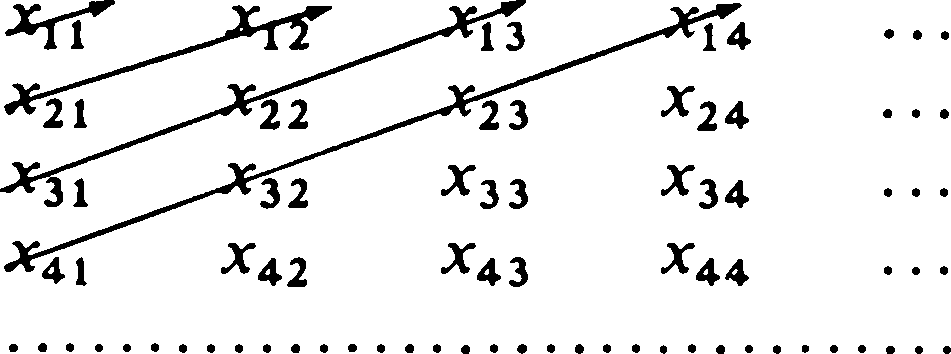
\includegraphics[scale = 0.15]{02/figures/eq2.16}}\label{eq:2.16}
    \end{equation}
    in which the elements of \(E_n\) form the \(n\)th row. The array contains all elements of \(S\). As indicated by the arrows, these elements can be arranged in a sequence
    \begin{equation}
        x_{11};x_{21},x_{12};x_{31},x_{22},x_{13};x_{41},x_{32},x_{23},x_{14};\ldots\label{eq:2.17}
    \end{equation}
    If any two of the sets \(E_n\) have elements in common, these will appear more than once in \eqref{eq:2.17}. Hence there is a subset \(T\) of the set of all positive integers such that \(S\sim T\), which shows that \(S\) is at most countable (Theorem~\ref{theorem:2.1}). Since \(E_1\subset S\), and \(E_1\) is infinite, \(S\) is infinite, and thus countable.
\end{proof}

\begin{corollary}
    Suppose \(A\) is at most countable, and, for every \(\alpha\in A\), \(B_\alpha\) is at most countable. Put
    \begin{equation*}
        T=\bigcup_{\alpha\in A}B_\alpha.
    \end{equation*}
    Then \(T\) is at most countable.
\end{corollary}

For \(T\) is equivalent to a subset of \eqref{eq:2.15}.

\begin{theorem}\label{theorem:2.3}
    Let \(A\) be a countable set, and let \(B_n\) be the set of all \(n\)-tuples \(\left(a_1,\ldots,a_n\right)\), where \(a_k\in A\) (\(k=1,\ldots,n\)), and the elements \(a_1\), \ldots, \(a_n\) need not be distinct. Then \(B_n\) is countable.
\end{theorem}

\begin{proof}
    That \(B_1\) is countable is evident, since \(B_1=A\). Suppose \(B_{n-1}\), is countable (\(n=2,3,4,\ldots\)). The elements of \(B_n\) are of the form
    \begin{equation}
        \left(b,a\right)\qquad\text{(\(b\in B_{n-1}\), \(a\in A\))}.
    \end{equation}
    For every fixed \(b\), the set of pairs \(\left(b,a\right)\) is equivalent to \(A\), and hence countable. Thus \(B_n\) is the union of a countable set of countable sets. By Theorem~\ref{theorem:2.2}, \(B_n\) is countable.

    The theorem follows by induction.
\end{proof}

\begin{corollary}
    The set of all rational numbers is countable.
\end{corollary}

\begin{proof}
    We apply Theorem~\ref{theorem:2.3}, with \(n=2\), noting that every rational \(r\) is of the form \(\rfrac{b}{a}\), where \(a\) and \(b\) are integers. The set of pairs \(\left(a,b\right)\), and therefore the set of fractions \(\rfrac{b}{a}\), is countable.
\end{proof}

In fact, even the set of all algebraic numbers is countable (see Exercise~\ref{exercise:2.2}).

That not all infinite sets are, however, countable, is shown by the next theorem.

\begin{theorem}\label{theorem:2.4}
    Let \(A\) be the set of all sequences whose elements are the digits \(0\) and \(1\). This set \(A\) is uncountable.
\end{theorem}

The elements of \(A\) are sequences like \(1\), \(0\), \(0\), \(1\), \(0\), \(1\), \(1\), \(1\), \ldots.

\begin{proof}
    Let \(E\) be a countable subset of \(A\), and let \(E\) consist of the sequences \(s_1\), \(s_2\), \(s_3\), \ldots. We construct a sequence \(s\) as follows. If the \(n\)th digit in \(s_n\) is \(1\), we let the \(n\)th digit of \(s\) be \(0\), and vice versa. Then the sequence \(s\) differs from every member of \(E\) in at least one place; hence \(s\notin E\). But clearly \(s\in A\), so that \(E\) is a proper subset of \(A\).

    We have shown that every countable subset of \(A\) is a proper subset of \(A\). It follows that \(A\) is uncountable (for otherwise \(A\) would be a proper subset of \(A\), which is absurd).
\end{proof}

The idea of the above proof was first used by Cantor, and is called Cantor's diagonal process; for, if the sequences \(s_1\), \(s_2\), \(s_3\), \ldots\ are placed in an array like \eqref{eq:2.16}, it is the elements on the diagonal which are involved in the construction of the new sequence.

Readers who are familiar with the binary representation of the real numbers (base \(2\) instead of \(10\)) will notice that Theorem~\ref{theorem:2.4} implies that the set of all real numbers is uncountable. We shall give a second proof of this fact in Theorem~\ref{theorem:2.?}.
